\section{Description Of The Algorithm}
%Introduce the system model by explaining the FFAST (dual problem - IFFT) architecture and then describe the decoding algorithm - peeling (multiple matches case) and Product code approach (only one exact match case).      
In this section we propose an algorithm, with sample and time complexity that is sub-linear in $N$, to find the locations $\underline{\tau} = (\tau_1, \tau_2, \cdots \tau_L)$ in the string $\underline{x}$, where the string (query) $\underline{y}$ matches. This is achieved by computing the cross-correlation of $\xv$ and $\underline{y}$, $R_{XY}$ and finding the positions where there is a significant peak.

The cross-correlation $\RXYv = [R_{XY}[0], R_{XY}[1], \cdots, R_{XY}[N]] $ of $\xv$ and $\yv$ is defined as

\begin{equation}\label{eqn:Rxy_def}
R_{XY}[m] \ =  \ \sum_{i=1}^{N} x[m+i] ~ y[i], \ 0 \leq m \leq N   
\end{equation}

The main idea here is that $\RXYv$ is sparse (upto some noise) with dominant peaks at $L$ positions ($\tau$) where the strings match, and noise components at $N-L$ positions where the strings do not match.

\begin{equation} \label{eqn:RXY_sparse}
R_{XY}[m] \ = \left\{
\begin{array}{ll}
  & v_m , \ \ \  \text{if} \ m \in \mathcal{T} \\
  & n_m , \ \ \ m \in [N]-\mathcal{T}
\end{array} 
\right.  
\end{equation}
where, $ \mathcal{T}:=\{\tau_1, \tau_2, \cdots, \tau_L\}$, $M-K \leq v_m \leq M $ is the signal component and $n_m$ is the noise component that is induced due to correlation of two i.i.d. sequence of random variables each taking values from $\mathcal{A} := \{+1,-1\}$.

The $\RXYv$ can also be computed as shown below.  
 
\begin{equation}\label{eqn:Rxy_fourier}
  \RXYv = \underset{\text{ \RNum{3} } } {\mathcal{F}^{-1}} \ \{ \underset{\text{ \RNum{1} } }{  \mathcal{F}\{\xv\}}  \odot \ \underset{\text{ \RNum{2} } }{ \mathcal{F}\{\yv'\}}  \} 
\end{equation}
 
where $\mathcal{F}\{ . \}$ and $\mathcal{F}^{-1}\{ . \}$ refers to $N$-point discrete Fourier transform and its inverse respectively, $\odot$ is the point-wise multiplication operation and ${ y'[n]} = { y^{*}[-n]}$. 

 We exploit this property of sparsity to compute $\RXYv$ by using only a subset of samples from $\Xv = \mathcal{F}\{\xv\} $ and $\Yv' = \mathcal{F}\{\yv'\} $, each sampled at positions $l \in \mathcal{S}$, where $\mathcal{S} = \mathcal{S}_{1,1} \cup \mathcal{S}_{1,2} \cup \cdots \cup \mathcal{S}_{i,j} \cup  \mathcal{S}_{d,B} \subset \{ 0,1,\cdots ,N-1 \}$ and $\mathcal{S}_{i,j}$, $1 \leq i \leq d $ and  $1 \leq j \leq B $ are disjoint sets of size $|\mathcal{S}_{i,j}| \approxeq N^{1-\alpha}$ with periodic sample points from $[N]$ given by 
 
 \begin{equation}
 \label{eqn:sampling_sets}\mathcal{S}_b = \{s_j,\ s_j + f_i,\ s_j + 2f_i,\ \cdots s_j + \lfloor{\frac{N}{f_i} }\rfloor f_i \}
 \end{equation}
   where, $b = i\times j$, and $s_j$'s and $f_i$'s are constants chosen based on the requirements from Robust Sparse Inverse Fourier Transform (RSIDFT) framework described in Section~\ref{sec:RSIDFT}.

 As evident from Equation~\ref{eqn:Rxy_fourier}, our algorithm for computing $R_{XY}$ consists of three stages:

\begin{enumerate}
	\item[\RNum{1}] \textit{Computing the sketch of $\xv$}: 
	
	 We assume that the sketch of $\xv$, \ $ \Xv[l] = \mathcal{F}\{\xv\}$ is precomputed at positions $l \in \mathcal{S}$ and stored in a database.  
	
	\item[\RNum{2}] \textit{Computing the sketch of $\yv$}:
	
	 For every new query $\yv$, $ \Yv'[l]$ is computed at $l \in \mathcal{S}$. Naively, the FFT algorithm can be used to compute this with $O(N \log N)$ complexity. Since only a subset $\mathcal{S}$ of samples from $\Yv'$ is needed, this can be done by using a folding technique described below.
	 
	  The idea behind this folding technique is to induce aliasing in $\yv'$ and then taking a smaller point Fourier Transform to compute the sub-sampled version $\Yv'$. Aliasing is induced by folding the signal $\yv'$ into blocks of length $N^{1-\alpha}$ and adding them. The desired subsampling patterns in frequency domain are induced by multiplying $\yv'$ with suitable exponentials. Let us denote the aliased versions of $\yv'$ by $\underline{y^{a}_{i,j}}'$. Then, $\underline{y^{a}_{i,j}}'$ is given by
	  \begin{equation}
	  	{y^{a}_{i,j}}'[p] = \sum \limits_{m = 0}^{\lfloor{\frac{N}{f_i}}\rfloor} y'[p + mf_i] e^{j \frac{2 \pi s_j}{N} } 
	  \end{equation}
	  Taking $\frac{N}{f_i}$ point DFT of $\underline{y^{a}_{i,j}}'$ produces $\Yv'[l]$ sub-sampled at $l \in \mathcal{S}_{i,j}$. To obtain all the samples in $\mathcal{S}$, the folding procedure needs to be carried out $dB$ times, once for each $(i,j)$ pair, where $1 \leq i \leq d $ and  $1 \leq j \leq B $.  
	       
	\item[\RNum{3}] \textit{Computing sparse $\mathcal{F}^{-1}$}: 
	
	 Since $R_{XY}$ is sparse, we use a Robust Sparse Inverse  Discrete Fourier Transform(RSIDFT) framework to compute the $L$-sparse coefficients. The architecture of RSIDFT is similar to FFAST proposed in \cite{pawar2014robust}, but the decoding algorithm has some key modifications to handle the noise model induced in this problem.
	 
	 
	 \subsection{RSIDFT Framework} 	\label{sec:RSIDFT}
	
	  Let $ \Zv  =  \Xv \odot \Yv'$ be the input to RSIDFT framework. The RSIDFT framework computes the $L$ dominant coefficients of $\zv$ $= {\RXYv}$ by using only a subsampled version of $\Zv$, $Z[l]$ at positions $l \in \mathcal{S}$.\\
	  Let $N = P_1 \times P_2 \times \cdots P_d$ be the prime factorization of $N$, the length of signals $\bf x \ \text{and} \ y$. For a given $\alpha$, we choose distinct $f_i = \prod P_j$, $i \in [d]$ such that $f_i \approxeq N^{\alpha} $. 
	 
	 Consider the RSIDFT framework shown in Figure~\ref{fig:rsidft}. The framework consists of $d-$stages, each with a different sub-sampling factor $f_i$. In each stage, there are $B$ branches with shifts from $\underline{s}$$\ = [s_1, s_2, \cdots s_B] $, with $s_1 =0$ in the first branch, and the rest chosen randomly from $[A]$. We can also carefully choose the shifts to satisfy Mutual Coherence property and Restricted Isometric property described in the analysis section.
	 
	 \begin{figure}
	 	\begin{center}
	 		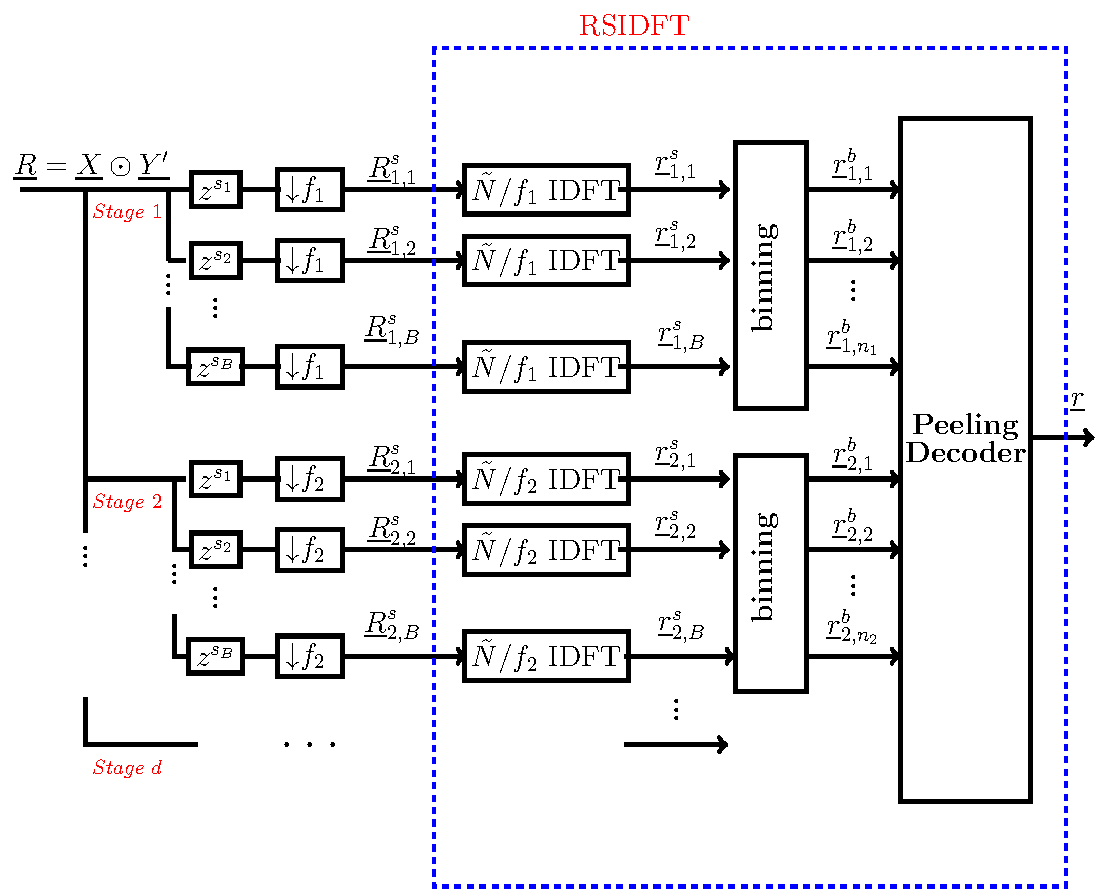
\includegraphics[height=7cm]{Figures/FFAST_Robust} 
	 	\end{center}	   
	 	\caption{ RSIDFT Framework to compute inverse Fourier Transform of a signal $\bf \hat{z}$ that is sparse in time domain. }\label{fig:rsidft}
	\vspace{5 pt}
	 \end{figure}	
	        
	
	 
	 Given the inputs $\Zv$, in branch $j$ of $i$th stage RSIDFT sub-samples the signal $\Zv$ at $\mathcal{S}_{i,j} = \{s_j,\ s_j + f_i,\ s_j + 2f_i,\ \cdots s_j + \lfloor{\frac{N}{f_i} }\rfloor f_i$, to obtain $\Zv^{s}_{i,j}$. Sub-sampling is followed by a $\frac{N}{f_i}-$ point IDFT in each branch of stage $i$ to obtain $ \zv^{s}_{i,j}$. Notice that $ \zv^{s}_{i,j}$ is an aliased version of $\zv$. \\
	 Let $\zv^{b}_{i,p_i}$ be the observations that is formed by combining all $p_i$th coefficients of $\zv^{s}_{i,j}$ (belonging to stage $i$) together as a vector, where $1 \leq p_i \leq \frac{N}{f_i}$.
	 
	 \[ \zv^{b}_{i,p_i} = \begin{bmatrix}
	 z^{s}_{i,1}[p_i] \\
	 z^{s}_{i,2}[p_i] \\
	 \vdots\\
	 z^{s}_{i,B}[p_i]
	 \end{bmatrix}  \]
	 
	  A peeling decoder takes these observations $ \zv^{b}_{i,p_i}$ as inputs and computes the sparse $\RXYv$.
	 
	 \subsection{Peeling Decoder}
		
	 Each coefficient of $\underline{z^{b}_{i,p_i}}$ is a bin that has $N^{\alpha}$ coefficients from $\RXYv$ hashed into it. This can be seen using a Tanner graph with $\RXYv$ as the left nodes (bit nodes) and the aliased coefficients  $\underline{z^{b}_{i,p_i}}$ as the right nodes (check-nodes). Notice that each bit node has degree $d$ and each check-node degree is approximately $N^{\alpha}$. The peeling decoder has the following three steps in the decoding process.
		 \begin{itemize}
		 	\setlength{\itemindent}{.1in}
			 \item \textit{Bin Identification :} In this step a check-node is classified as a Zero-ton ($degree = 0$) or a Single-ton ($degree = 1)$ or a Multi-ton ($degree >1$). The classification is done based on a comparing the first observation,$z^{b}_{i,p_i}[1]$ (corresponding to zero shift), with a predefined threshold. The threshold is set differently for Exact Matching and Approximate Matching cases.\\
			 {\bf Exact Matching:} 
			                \[
			                \begin{array}{ll}
			                \text{Zero-ton:}& \ \ z^{b}_{i,p_i}[1] < M/2 \\
			                \text{Single-ton:}& \ \ M/2 \leq z^{b}_{i,p_i}[1] \leq 3M/2 \\ 
			                \text{Multi-ton:}& \ \ z^{b}_{i,p_i}[1] > 3M/2
			                \end{array}
			                \]   
			                
			 {\bf Approximate Matching:} 
			 \[
			 \begin{array}{ll}
			 \text{Zero-ton:}& \ \ z^{b}_{i,p_i}[1] < \frac{(1-3\eta/2)M}{2} \\ 
			 \text{Single-ton:}& \ \ \frac{(1-3\eta/2)M}{2} < z^{b}_{i,p_i}[1] < \frac{(1-\eta/2)3M}{2}   \\
			 \text{Double-ton:}& \ \ \frac{(1-\eta/2)3M}{2} < z^{b}_{i,p_i}[1] < \frac{(5-3\eta)M}{2}\\ 
			 \text{Multi-ton:}& \ \ z^{b}_{i,p_i}[1] > \frac{(5-3\eta)M}{2}\\
			 \end{array}
			 \] 
			   
			 \item \textit{Position Identification :} Given that a check-node is classified as a Single-ton, we need to identify the position of the non-zero coefficient  hashed into it. This is done by correlating the observation vector $\underline{z^{b}_{i,p_i}}$ with each column of $S = [\underline{s_1} \ \underline{s_2} \cdots \underline{s_A}]$ and then picking the column index, $p'$ that produced the maximum value.
			 \[ p' = \underset{l}{\argmax}\  \underline{s^T_l} ~ \underline{z^{b}_{i,p_i}}\]
			 
			 \item \textit{Peeling Process: } Although the main idea behind the peeling process is same for Exact Matching and the Approximate Matching scenarios, there is some minor differences in their implementation. The main idea here is to find the Singletons and then remove its contribution from other check-nodes where the bit-node corresponding to this Singleton participates.
			 
			 
			  {\bf Exact Matching:} Here we remove the identified Singleton's contribution from all the check-nodes it participates in.
			  
			  {\bf Approximate Matching:} Here we only remove the identified Singleton's contribution from a double-ton and do not alter multi-tons whose $degree > 2$.
			  		 
		 \end{itemize} 
	 
	 
\end{enumerate}	
	 
	  
	 
	 

